\documentclass{beamer}

\title{PageRank}
\author{Ben Burns, Dan Magazu, Lucas Chagas, \\Thomas Webster, Trung Do}
\date{Fall 2021}

\usepackage{outlines}
\usepackage{graphicx}
\usepackage{amsmath}
\usepackage{color, xcolor, mdframed}
\usepackage{hyperref}
\hypersetup{
    colorlinks=true,
    linkcolor=blue,
    filecolor=blue,      
    urlcolor=blue,
    pdfpagemode=FullScreen,
}

\graphicspath{{./images}}

\addtobeamertemplate{navigation symbols}{}{
    \usebeamerfont{footline}
    \usebeamercolor[fg]{footline}
    \hspace{1em}
    \insertframenumber/\inserttotalframenumber
}

%\AtBeginSection[ ]
%{
%\begin{frame}{Outline}
%    \tableofcontents[currentsection]
%\end{frame}
%}

\begin{document}

\frame{\titlepage}

\begin{frame}
\frametitle{Table of Contents}
\tableofcontents
\end{frame}


\section{Motivation \& History}
\begin{frame}[t]
\frametitle{Motivation}
\begin{itemize}
    \setlength\itemsep{0.5em}
    \item Problem: the internet has a \emph{lot} of web pages
    \item A lot of the information out there either isn't relevant to us, or is inaccurate
    \item Motivation: we want a program that, when provided a phrase, returns webpages with information relevant to the input
    \item Intuitive solution: return back websites that either contain that phrase, or contain similar phrases
    \item This helps us find more \emph{relevant} pages, but we can't know if we're getting the best information (much less \emph{accurate} information) without manually going through each result
    \item We desire a stronger solution
\end{itemize}
\end{frame}

\begin{frame}[t]
\frametitle{PageRank}
\begin{outline}
    \1 Invented by Sergey Brin and Larry Page (1998)\footnotemark 
        \2 Publication marks them becoming co-founders of Google  
    \1 Idea: we want some way to numerically discern how important each webpage is
    \1 PageRank: the procedure for scoring each website
    \1 Google: the database that indexes the PageRank of each website for search
    \1 Everytime Google crawls the web to reindex, it recalculates the PageRank scores for all webpages
\end{outline}
\footnotetext[1]{Many use the year of the original manuscript, 1996}
\end{frame}

\begin{frame}[t]{The Big Idea behind PageRank}
\begin{outline}
    \1 PageRank is an algorithm to determine the importance of a website relatively to all other websites. The algorithm ranks the importance of website $w,$ i.e., PR($w$), based on the number of links points to website w and the \emph{quality} of each pointing link from the other source website. 

    \1 \textbf{The underlying assumption}: More important website are likely to receive more links from other website. Since the algorithm measures the relative popularity ("ranking") between all websites, websites with higher ranking score are ranked higher. The sum of all ranking score equals 1 (will see why later).
\end{outline}
\end{frame}

\begin{frame}{Visulization of PageRank score}
    \begin{center}
        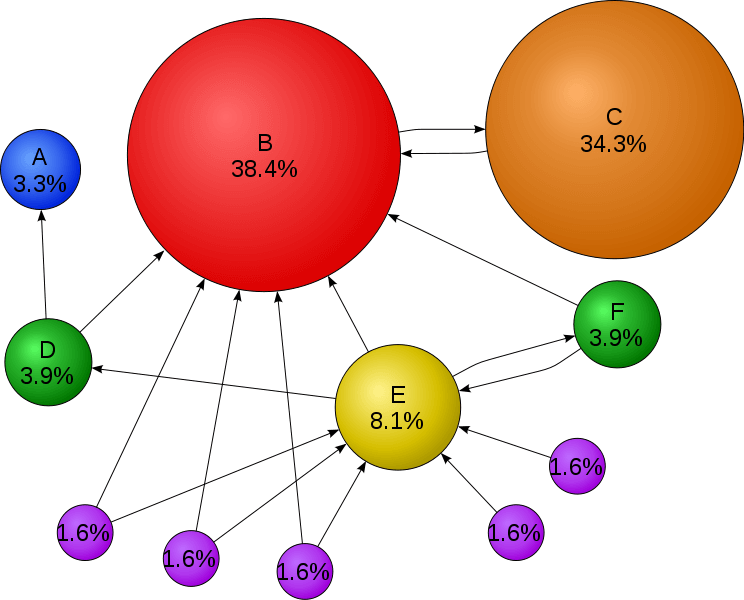
\includegraphics[width=0.9\textwidth]{pagerankexample.png}
    \end{center}
\end{frame}

\section{Formalizing PageRank}
\begin{frame}[t]{Formalizing the PageRank problem}
\begin{outline}
    \1 As a graph: Each website is represented by a node assigned with a PageRank value, denoted by PR(w). 
    \1 If a website w has a link to another website v (meaning there are an outbound link from w and an inbound link to v), then there is a directed edge from node w to node v. 
    \1 Multiple links from w to v is treated as a single edge from node w to v, and all self-links from a website to itself are ignored. \textbf{Thus, this is a node-weighted, simple, no self-loop directed graph}.
\end{outline}
\begin{center}
    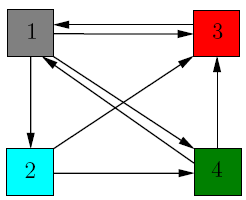
\includegraphics[width=0.4\textwidth]{unweighted.png}
\end{center}
\end{frame}

\begin{frame}
\frametitle{Add Weight to Edges}
        \begin{outline}
            \1 An edge from $u$ to $v$ will "transfer" the score from node $u$ to node $v$ an amount of PR($u$)/O($u$), where PR($u$) is the current score of $u$, and O($u$) is the total number of outlinks of node $u$.  Thus, PR($v$) += PR($w$)/L($w$). 
            \1 In another words, for a given node in the graph:
            \1 \textbf{An outbound link} will "give" away the PR value of the source node to the recipient node.  
            \1 \textbf{An inbound link} will add the PR value from the source node to the recipient node.
        \end{outline}

\begin{center}
    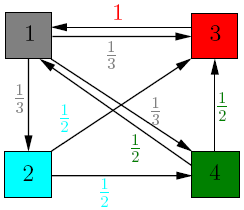
\includegraphics[width= 0.4\textwidth]{weighted.png}
\end{center}
\end{frame}

\begin{frame}[t]{Formulate the transition matrix $A$}
    \begin{columns}
        \begin{column}{0.5\textwidth}
            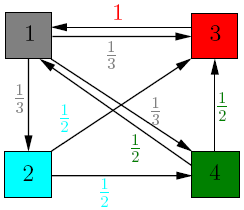
\includegraphics[width=\textwidth]{weighted.png}
        \end{column}
        \begin{column}{0.5\textwidth}
            \bgroup
            \renewcommand*{\arraystretch}{2}
            \begin{math}
                A = \begin{bmatrix}
                    0 & 0 & 1 & \dfrac{1}{2}\\
                    \dfrac{1}{3} & 0 & 0 & 0\\
                    \dfrac{1}{3} & \dfrac{1}{2} & 0 & \dfrac{1}{2}\\
                    \dfrac{1}{3} & \dfrac{1}{2} & 0 & 0\\
                \end{bmatrix}
            \end{math}
            \egroup
        \end{column}
    \end{columns}
    \begin{outline}
        \1 Notice some special properties of matrix A: 
        \2 All entries of A are non-negative. 
        \2 If there is an outlink from node $w$, then the column  corresponding to node $w$ has the sum of its entries equals 1. Otherwise, the sum equals 0.
        \1  Matrix A is called a \textbf{\emph{column stochastic matrix}} (all matrix entries are non-negative and the sum of 
         the entries in every column is 1). 
    \end{outline}
\end{frame}

\section{Ways to Interpret PageRank}
%\begin{frame}[t]{Perspectives for Solving}
%    \begin{itemize}
%        \setlength\itemsep{1em}
%        \item There are two ways to understand the problem:
%        \item[1)] as an Eigenvector problem
%        \item[2)] as a probability problem
%        \item Both perspectives use linear algebra 
%    \end{itemize}
%\end{frame}

\subsection{Eigenvector Approach}
\begin{frame}[t]{Translate PageRank Problem into an Eigenvector Problem}
    \begin{outline}
        \1 Let us denotes vector v with each entry of the vector as the PageRank value of the corresponding nodes: 
        \begin{center}
            $v = \begin{bmatrix}
                x_1\\
                x_2\\
                x_3\\
                x_4\\
            \end{bmatrix}$
        \end{center}
        \1 Analyzing the relationship between 4 nodes in the example we get the system 
        \begin{center}
            $\begin{cases}
                x_1 = 1 \cdot x_3 + \dfrac{1}{2}\cdot x_4&\\[6pt]
                x_2 = \dfrac{1}{3}\cdot x_1&\\[6pt]
                x_3 = \dfrac{1}{3}\cdot x_1 + \dfrac{1}{2}\cdot x_2 + \dfrac{1}{2}\cdot x_4&\\[6pt]
                x_4 = \dfrac{1}{3}\cdot x_1 + \dfrac{1}{2}\cdot x_2&\\[6pt]
            \end{cases}$
        \end{center}
    \end{outline}
\end{frame}

\begin{frame}[t]{Eigenvector Problem (cont.)}
\begin{outline}
    \1 Thus we can translate the problem into the eigenvector problem:
    \begin{align*}
        A\cdot \begin{bmatrix}
            x_1\\
            x_2\\
            x_3\\
            x_4\\
        \end{bmatrix} &= \begin{bmatrix}
            x_1\\
            x_2\\
            x_3\\
            x_4\\
        \end{bmatrix}
    \end{align*}
\end{outline}
\end{frame}



%\begin{frame}[t]{Solving for Eigenvector}
%    \begin{outline}
%            \2 Find an eigenvector $v$ corresponding to the eigenvalue 1 of the following system:
%    \end{outline}
%\end{frame}

\begin{frame}[t]{Continue Solving}
\begin{outline}
    \1 The conditions to rigorously use the eigenvector method will be defined below. For now, we can solve for the eigenvector corresponding to the eigenvalue 1:
    \begin{align*}
        c\cdot \begin{bmatrix}
            12\\ 4\\ 9\\ 6\\
        \end{bmatrix}
    \end{align*}
    \1 Every vector in the above format is the eigenvector corresponding to eigenvalue 1. 
\end{outline}
\end{frame}

\begin{frame}[t]{Continue Solving (cont.)}
    \begin{outline}
        \1 We choose $c$ such that the sum of all entries in this vector equals 1 (we later refer to it as "the probabilistic eigenvector corresponding to the eigenvalue 1")
        \begin{center}
            \begin{math}
                \dfrac{1}{31}\cdot \begin{bmatrix}
                    12 \\ 4 \\ 9 \\ 6\\
                \end{bmatrix} \sim \begin{bmatrix}
                    0.38 \\ 0.12 \\ 0.29 \\ 0.19\\
                \end{bmatrix}
            \end{math} is our PageRank vector
        \end{center}
    \end{outline}
\end{frame}

\begin{frame}[t]{Power Iteration Method}
    \begin{outline}
        \1 Want to determine the eigenvector of the square matrix $A$
        \1 Start out with 
        \begin{center}
            $\vec{v_0} = \begin{bmatrix}
                0.25 \\ 0.25 \\ 0.25 \\ 0.25 \\
            \end{bmatrix}$
        \end{center}
        as a candidate eigenvector corresponding to eigenvalue of 1
        \1 Calculate $\vec{v_1} = A\vec{v_0}$ to get a new vector
        \1 Continue to iterate until $v_k$ converges (if it does as at all)
    \end{outline}
\end{frame}

\begin{frame}{A few questions to ask$\ldots$}
\Large\begin{itemize}
    \setlength\itemsep{2em}
    \item Will $v_k$ always converge?
    \item Will $v_k$ give us any useful information about the ranking of websites?
\end{itemize}    
\end{frame}

\subsection{Random Walk Interpretation}
\begin{frame}[t]{Random Walk Interpretation}
    \begin{outline}
        \1 Consider someone browsing the web who is randomly clicking on links. We refer to this person as the "random walker" 
        \1 Interpret our rank vector $r$ as a probability distribution $p(t)$ where $t$ is time
        \1 $p(t) = \left[ \dfrac{1}{N}, \dfrac{1}{N}, \ldots, \dfrac{1}{N} \right]^T$ is a vector where at some time $t$ the $i^{th}$ index represents the probability that the random walker is at page $i$.
        \1 To predict where the random walker is at time $t + 1$ we calculate $Mp(t) = p(t + 1)$
    \end{outline}
\end{frame}

\begin{frame}[t]{Random Walk Interpretation}
\begin{outline}
    \1 Suppose that for some $t$ we find that $Mp(t) = p(t)$
    \1 In other words, we have found a steady state distribution!
    \1 We recognize this as a Markov process where the probability that the random walker is in a given page at some time $t$ is solely determined by what our probability distribution looked like at time $t-1$
    \1 From Markov theory, we know that the transition matrix $M$ needs to follow a few characteristics for $p(t)$ to converge to a unique vector
    \1 What constraints do we need to apply to $M$ so that the power iteration algorithm will always converge?
\end{outline}   
\end{frame}

\begin{frame}[t]{When Power Iteration Fails}
    \begin{outline}
        \1 Before discussing constaints on $M$ we need to observe the cases where power iteration either fails to converge or produces a nonsense result
        \1 So far, we have gone along with the formulation of PageRank where the importance of a webpage depends on its incoming links
        \1 We haven't taken the time to consider if this approach even makes sense
        \1 Consider two problems that arise:
            \2 Spider Traps
            \2 Dead Ends
    \end{outline}
\end{frame}
\section{Treating Problematic Edge Cases}
\begin{frame}[t]{Spider Traps}
\begin{outline}
    \1 Our random walker gets stuck in a portion of the graph leading to most of the “importance” to flow into subgraph where the walker is stuck
    \1 Example: what happens when we run power iteration on this web graph? (notice that the random walker will get stuck on page $m$)
    \begin{center}
        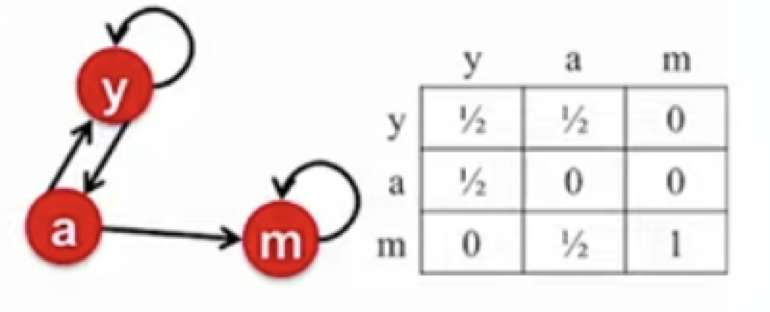
\includegraphics[width=0.6\textwidth]{spider.png}
    \end{center}
\end{outline}
\end{frame}

\begin{frame}[t]{Spider Trap Continued}
\begin{outline}
    \1 Power iteration successfuly converges! So we're done right?
    \1 Wrong. Page $m$ receives a rank of $r_m = 1$ while the rest of the pages are of no importance
    \1 From the random walker's perspective this makes sense. But this is not what we want.
    
    \begin{center}
        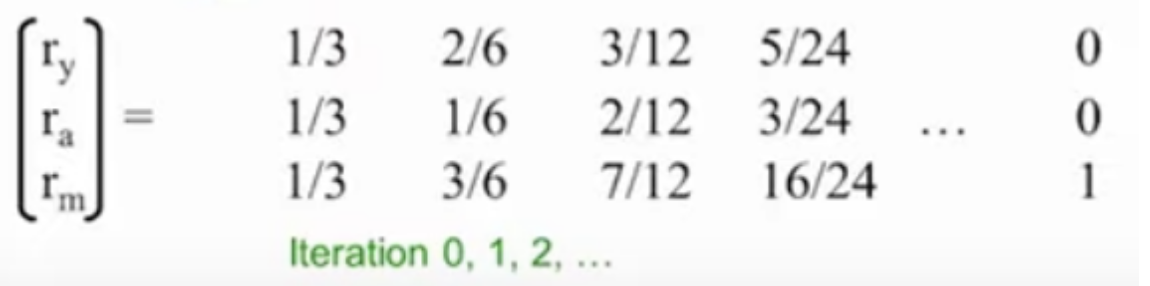
\includegraphics[width=0.8\textwidth]{spider1b.png}
    \end{center}
\end{outline}
\end{frame}
\begin{frame}{Another Spider Trap}
\begin{columns}
    \begin{column}{0.5\textwidth}
        \parskip=1em
        Another example:

    Page a starts with an importance
    of 1 and passes it page $b$ in the first
    iteration. Then $b$ passes 1 to $a, \cdots$
    And this process continues 
    indefinitely.

    We fail to converge!
    \parskip=0em
    \end{column}
    \begin{column}{0.5\textwidth}
        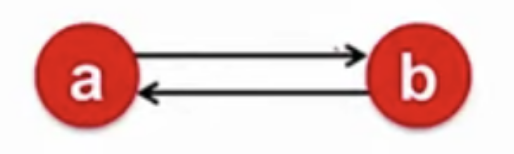
\includegraphics[width=\textwidth]{spider2a.png}    
        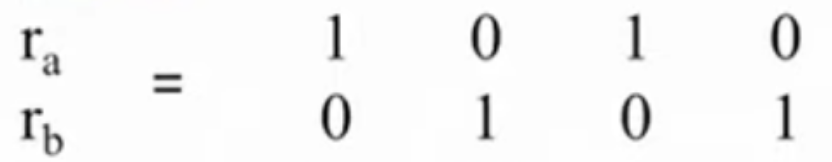
\includegraphics[width=\textwidth]{spider2b.png}    
    \end{column}
\end{columns}
\end{frame}
\begin{frame}[t]{The Solution to the Spider Traps}
    \begin{itemize}
        \item At each iteration, we give the random walker the option to either continue following outbound links or to randomly "teleport" to another page on the web
        \item We denote the probability that the user clicks a link by $\beta$, and the probability of teleporting by 1 -$\beta$
        \item Now our random walkers can't get stuck in a subgraph of our web, and we avoid having a subset of pages hog all of the "importance" value
    \end{itemize}
\end{frame}
    
\begin{frame}[t]{Dead Ends}
\begin{columns}
    \begin{column}{0.5\textwidth}
        \begin{outline}
            \1 The random walker encounters a web page without any outbound links leaving them nowhere to go.
            \1 Example:
            We converge but power iteration
            tells us that both page a and b are
            unimportant!
        \end{outline}
    \end{column}
    \begin{column}{0.5\textwidth}
        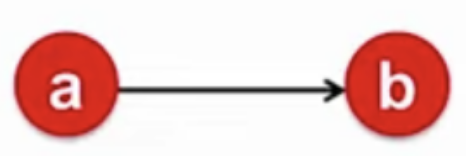
\includegraphics[width=\textwidth]{deadenda.png}
        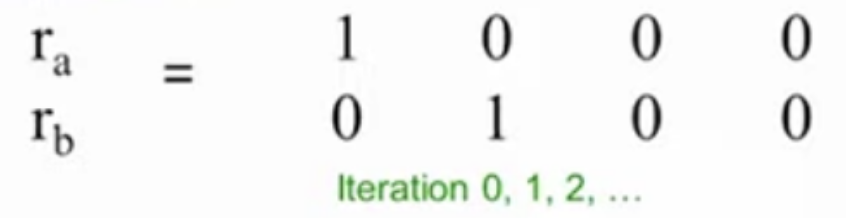
\includegraphics[width=\textwidth]{deadendb.png}
    \end{column}
\end{columns}
\end{frame}
\begin{frame}[t]{The Solution to Dead Ends}
\begin{outline}
\1 If our random walker encounters a page with no outbound links, we immediately teleport them to a random web page
\1 Example:

\begin{center}
    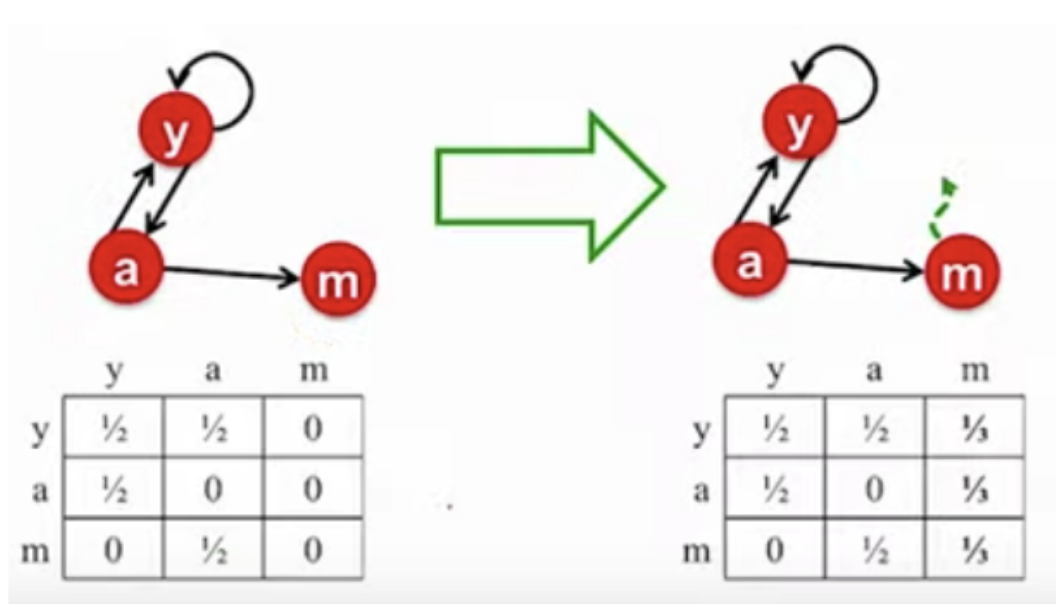
\includegraphics[width=0.7\textwidth]{desol.png}
\end{center}
\end{outline}
\end{frame}
    
\begin{frame}[t]{Do Teleports Solve Convergence?}
\begin{outline}
\1 Yes. In fact, after dealing with spider traps and dead ends, the power iteration algorithm will always converge
\1 Recall that power iteration is simply a Markov process where if matrix $M$ has special characteristics it will always converge
\1 Markov theory tells us that if $M$ is stochastic, aperiodic, and irreducible, then it will always converge to a unique, positive, stationary vector
\end{outline}
\end{frame}
   
\begin{frame}[t]{Stochastic}
\begin{outline}
    \1 Every column in the transition matrix must sum to 1
    \1 When initially constructing our adjacency matrix $A$, if a page has no outbound links (dead end) then the entire column would sum up to 0.
    \1 Our solution to deadends guarantees that every column adds up to 1.
\end{outline}
\end{frame}

\begin{frame}[t]{Aperiodic}
\begin{outline}
    \1 A chain is periodic if there exist $k > 1$ such that the interval between two visits to some state s is always a multiple of $k$
    \1 Our solution to spider traps also introduces self-loops into the graph 
    \1 This turns the graph aperiodic
    
    \begin{center}
        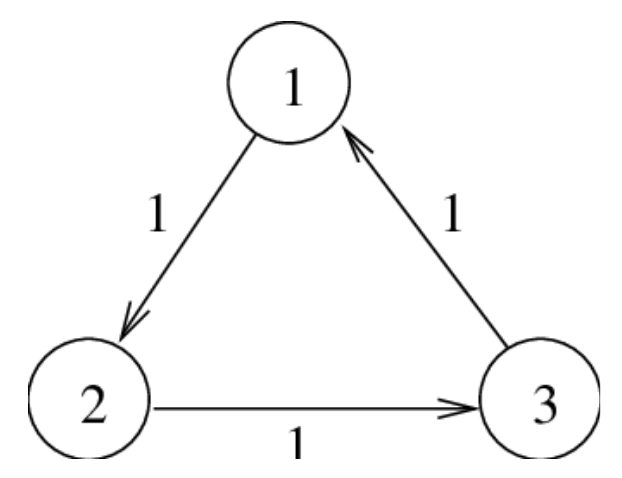
\includegraphics[width=0.6\textwidth]{aperiodic.png}
    \end{center}

\end{outline}

\end{frame}

\begin{frame}[t]{Irreducible}
\begin{outline}
    \1 Irreducible: From any state, there is a non-zero probability of going from any one state to another
    \1 Our solution to spider traps gives the random walker the opportunity to randomly jump to any page in the web graph
    \1 Therefore, we will always be able to navigate 
\end{outline}
\end{frame}

\begin{frame}[t]{The PageRank equation}
\begin{outline}
\1 Google's solution makes the Markov Transition matrix stochastic, aperiodic, and irreducible.

\1 PageRank equation:

\begin{mdframed}[backgroundcolor=blue!20]
    \begin{center}
        $r_j = \sum\limits_{i\to j}\beta \dfrac{r_i}{d_i} + (1-\beta)\dfrac{1}{n}$
    \end{center}
\end{mdframed}

\2 The summation is the sum of all of the importance of node $I$ that point to it where $r_j$ and $r_i$ is the probability that the random surf is on this node.
\2 This is divided by $d_i$, which is the probability that the random surf traverses the link when iterating towards $j$. This only happens with probability $\beta$, when the surfer decides to follow the link.
\2 The $(1-\beta)/n$ represents when the random walkers decide to jump somewhere else, using the probability ($1-\beta) \cdot 1/n$, where $n$ is the number of nodes in the entire network.
\end{outline}
\end{frame}

\section{Google's Implementation}
\begin{frame}[t]{The Google Matrix}
    \begin{mdframed}[backgroundcolor=blue!20]
        \begin{center}
            $A = \beta M + (1-\beta)\dfrac{1}{n}e\cdot e^T$
        \end{center}
    \end{mdframed}
    \begin{itemize}
       
        \item Matrix A, also known as the google matrix, is the transition matrix multiplied with ß(for random jumps) plus the probabilities due to random jumps, known as (1-ß). 
    
    
    \item This is then multiplied by e, the outer product of a vector that is of all 1s.
    \end{itemize}
    \end{frame}

\begin{frame}{Using the Google Matrix Example}
    \begin{center}
        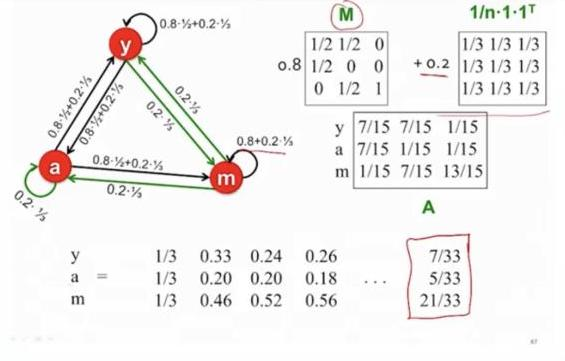
\includegraphics[width=\textwidth]{example.jpg}   
    \end{center}
\end{frame}

\begin{frame}[t]{Sources}
    \small
    \href{https://www.classes.cs.uchicago.edu/archive/2017/fall/12100-1/lecture-examples/PageRank/slides.pdf}{https://www.classes.cs.uchicago.edu/archive/2017/fall/12100-1/lecture-examples/PageRank/slides.pdf}\\
    \href{https://web.stanford.edu/class/cs246/slides/10-spam.pdf}{https://web.stanford.edu/class/cs246/slides/10-spam.pdf}\\
    \href{https://www.cs.rpi.edu/~slotag/classes/FA16/slides/lec04-web1.pdf}{https://www.cs.rpi.edu/~slotag/classes/FA16/slides/lec04-web1.pdf}\\
    \href{https://www.stat.cmu.edu/~ryantibs/datamining/lectures/03-pr.pdf}{https://www.stat.cmu.edu/~ryantibs/datamining/lectures/03-pr.pdf}\\
    \href{https://www.ccs.neu.edu/home/daikeshi/notes/PageRank.pdf}{https://www.ccs.neu.edu/home/daikeshi/notes/PageRank.pdf}\\
    \href{http://www.cs.sjsu.edu/faculty/pollett/masters/Semesters/Fall11/tanmayee/Deliverable3.pdf}{http://www.cs.sjsu.edu/faculty/pollett/masters/Semesters/Fall11/\\tanmayee/Deliverable3.pdf}\\
    \href{https://www.stat.uchicago.edu/~lekheng/meetings/mathofranking/ref/gleich.pdf}{https://www.stat.uchicago.edu/~lekheng/meetings/mathofranking/\\ref/gleich.pdf} \\
    \href{http://web.eecs.utk.edu/~roffutt/files/sp20ppts/PageRank.pdf}{http://web.eecs.utk.edu/~roffutt/files/sp20ppts/PageRank.pdf}\\
    \href{https://www.amsi.org.au/teacher_modules/pdfs/Maths_delivers/Pagerank5.pdf}{https://www.amsi.org.au/teacher\_modules/pdfs/Maths\_delivers/\\Pagerank5.pdf}\\
    \href{http://www.ams.org/publicoutreach/feature-column/fcarc-pagerank}{http://www.ams.org/publicoutreach/feature-column/fcarc-pagerank}\\
\end{frame}
\end{document}